\documentclass[11pt]{article}

    \usepackage[breakable]{tcolorbox}
    \usepackage{parskip} % Stop auto-indenting (to mimic markdown behaviour)
    
    \usepackage{iftex}
    \ifPDFTeX
    	\usepackage[T1]{fontenc}
    	\usepackage{mathpazo}
    \else
    	\usepackage{fontspec}
    \fi

    % Basic figure setup, for now with no caption control since it's done
    % automatically by Pandoc (which extracts ![](path) syntax from Markdown).
    \usepackage{graphicx}
    % Maintain compatibility with old templates. Remove in nbconvert 6.0
    \let\Oldincludegraphics\includegraphics
    % Ensure that by default, figures have no caption (until we provide a
    % proper Figure object with a Caption API and a way to capture that
    % in the conversion process - todo).
    \usepackage{caption}
    \DeclareCaptionFormat{nocaption}{}
    \captionsetup{format=nocaption,aboveskip=0pt,belowskip=0pt}

    \usepackage{float}
    \floatplacement{figure}{H} % forces figures to be placed at the correct location
    \usepackage{xcolor} % Allow colors to be defined
    \usepackage{enumerate} % Needed for markdown enumerations to work
    \usepackage{geometry} % Used to adjust the document margins
    \usepackage{amsmath} % Equations
    \usepackage{amssymb} % Equations
    \usepackage{textcomp} % defines textquotesingle
    % Hack from http://tex.stackexchange.com/a/47451/13684:
    \AtBeginDocument{%
        \def\PYZsq{\textquotesingle}% Upright quotes in Pygmentized code
    }
    \usepackage{upquote} % Upright quotes for verbatim code
    \usepackage{eurosym} % defines \euro
    \usepackage[mathletters]{ucs} % Extended unicode (utf-8) support
    \usepackage{fancyvrb} % verbatim replacement that allows latex
    \usepackage{grffile} % extends the file name processing of package graphics 
                         % to support a larger range
    \makeatletter % fix for old versions of grffile with XeLaTeX
    \@ifpackagelater{grffile}{2019/11/01}
    {
      % Do nothing on new versions
    }
    {
      \def\Gread@@xetex#1{%
        \IfFileExists{"\Gin@base".bb}%
        {\Gread@eps{\Gin@base.bb}}%
        {\Gread@@xetex@aux#1}%
      }
    }
    \makeatother
    \usepackage[Export]{adjustbox} % Used to constrain images to a maximum size
    \adjustboxset{max size={0.9\linewidth}{0.9\paperheight}}

    % The hyperref package gives us a pdf with properly built
    % internal navigation ('pdf bookmarks' for the table of contents,
    % internal cross-reference links, web links for URLs, etc.)
    \usepackage{hyperref}
    % The default LaTeX title has an obnoxious amount of whitespace. By default,
    % titling removes some of it. It also provides customization options.
    \usepackage{titling}
    \usepackage{longtable} % longtable support required by pandoc >1.10
    \usepackage{booktabs}  % table support for pandoc > 1.12.2
    \usepackage[inline]{enumitem} % IRkernel/repr support (it uses the enumerate* environment)
    \usepackage[normalem]{ulem} % ulem is needed to support strikethroughs (\sout)
                                % normalem makes italics be italics, not underlines
    \usepackage{mathrsfs}
    

    
    % Colors for the hyperref package
    \definecolor{urlcolor}{rgb}{0,.145,.698}
    \definecolor{linkcolor}{rgb}{.71,0.21,0.01}
    \definecolor{citecolor}{rgb}{.12,.54,.11}

    % ANSI colors
    \definecolor{ansi-black}{HTML}{3E424D}
    \definecolor{ansi-black-intense}{HTML}{282C36}
    \definecolor{ansi-red}{HTML}{E75C58}
    \definecolor{ansi-red-intense}{HTML}{B22B31}
    \definecolor{ansi-green}{HTML}{00A250}
    \definecolor{ansi-green-intense}{HTML}{007427}
    \definecolor{ansi-yellow}{HTML}{DDB62B}
    \definecolor{ansi-yellow-intense}{HTML}{B27D12}
    \definecolor{ansi-blue}{HTML}{208FFB}
    \definecolor{ansi-blue-intense}{HTML}{0065CA}
    \definecolor{ansi-magenta}{HTML}{D160C4}
    \definecolor{ansi-magenta-intense}{HTML}{A03196}
    \definecolor{ansi-cyan}{HTML}{60C6C8}
    \definecolor{ansi-cyan-intense}{HTML}{258F8F}
    \definecolor{ansi-white}{HTML}{C5C1B4}
    \definecolor{ansi-white-intense}{HTML}{A1A6B2}
    \definecolor{ansi-default-inverse-fg}{HTML}{FFFFFF}
    \definecolor{ansi-default-inverse-bg}{HTML}{000000}

    % common color for the border for error outputs.
    \definecolor{outerrorbackground}{HTML}{FFDFDF}

    % commands and environments needed by pandoc snippets
    % extracted from the output of `pandoc -s`
    \providecommand{\tightlist}{%
      \setlength{\itemsep}{0pt}\setlength{\parskip}{0pt}}
    \DefineVerbatimEnvironment{Highlighting}{Verbatim}{commandchars=\\\{\}}
    % Add ',fontsize=\small' for more characters per line
    \newenvironment{Shaded}{}{}
    \newcommand{\KeywordTok}[1]{\textcolor[rgb]{0.00,0.44,0.13}{\textbf{{#1}}}}
    \newcommand{\DataTypeTok}[1]{\textcolor[rgb]{0.56,0.13,0.00}{{#1}}}
    \newcommand{\DecValTok}[1]{\textcolor[rgb]{0.25,0.63,0.44}{{#1}}}
    \newcommand{\BaseNTok}[1]{\textcolor[rgb]{0.25,0.63,0.44}{{#1}}}
    \newcommand{\FloatTok}[1]{\textcolor[rgb]{0.25,0.63,0.44}{{#1}}}
    \newcommand{\CharTok}[1]{\textcolor[rgb]{0.25,0.44,0.63}{{#1}}}
    \newcommand{\StringTok}[1]{\textcolor[rgb]{0.25,0.44,0.63}{{#1}}}
    \newcommand{\CommentTok}[1]{\textcolor[rgb]{0.38,0.63,0.69}{\textit{{#1}}}}
    \newcommand{\OtherTok}[1]{\textcolor[rgb]{0.00,0.44,0.13}{{#1}}}
    \newcommand{\AlertTok}[1]{\textcolor[rgb]{1.00,0.00,0.00}{\textbf{{#1}}}}
    \newcommand{\FunctionTok}[1]{\textcolor[rgb]{0.02,0.16,0.49}{{#1}}}
    \newcommand{\RegionMarkerTok}[1]{{#1}}
    \newcommand{\ErrorTok}[1]{\textcolor[rgb]{1.00,0.00,0.00}{\textbf{{#1}}}}
    \newcommand{\NormalTok}[1]{{#1}}
    
    % Additional commands for more recent versions of Pandoc
    \newcommand{\ConstantTok}[1]{\textcolor[rgb]{0.53,0.00,0.00}{{#1}}}
    \newcommand{\SpecialCharTok}[1]{\textcolor[rgb]{0.25,0.44,0.63}{{#1}}}
    \newcommand{\VerbatimStringTok}[1]{\textcolor[rgb]{0.25,0.44,0.63}{{#1}}}
    \newcommand{\SpecialStringTok}[1]{\textcolor[rgb]{0.73,0.40,0.53}{{#1}}}
    \newcommand{\ImportTok}[1]{{#1}}
    \newcommand{\DocumentationTok}[1]{\textcolor[rgb]{0.73,0.13,0.13}{\textit{{#1}}}}
    \newcommand{\AnnotationTok}[1]{\textcolor[rgb]{0.38,0.63,0.69}{\textbf{\textit{{#1}}}}}
    \newcommand{\CommentVarTok}[1]{\textcolor[rgb]{0.38,0.63,0.69}{\textbf{\textit{{#1}}}}}
    \newcommand{\VariableTok}[1]{\textcolor[rgb]{0.10,0.09,0.49}{{#1}}}
    \newcommand{\ControlFlowTok}[1]{\textcolor[rgb]{0.00,0.44,0.13}{\textbf{{#1}}}}
    \newcommand{\OperatorTok}[1]{\textcolor[rgb]{0.40,0.40,0.40}{{#1}}}
    \newcommand{\BuiltInTok}[1]{{#1}}
    \newcommand{\ExtensionTok}[1]{{#1}}
    \newcommand{\PreprocessorTok}[1]{\textcolor[rgb]{0.74,0.48,0.00}{{#1}}}
    \newcommand{\AttributeTok}[1]{\textcolor[rgb]{0.49,0.56,0.16}{{#1}}}
    \newcommand{\InformationTok}[1]{\textcolor[rgb]{0.38,0.63,0.69}{\textbf{\textit{{#1}}}}}
    \newcommand{\WarningTok}[1]{\textcolor[rgb]{0.38,0.63,0.69}{\textbf{\textit{{#1}}}}}
    
    
    % Define a nice break command that doesn't care if a line doesn't already
    % exist.
    \def\br{\hspace*{\fill} \\* }
    % Math Jax compatibility definitions
    \def\gt{>}
    \def\lt{<}
    \let\Oldtex\TeX
    \let\Oldlatex\LaTeX
    \renewcommand{\TeX}{\textrm{\Oldtex}}
    \renewcommand{\LaTeX}{\textrm{\Oldlatex}}
    % Document parameters
    % Document title
    \title{chapter-2-1}
    
    
    
    
    
% Pygments definitions
\makeatletter
\def\PY@reset{\let\PY@it=\relax \let\PY@bf=\relax%
    \let\PY@ul=\relax \let\PY@tc=\relax%
    \let\PY@bc=\relax \let\PY@ff=\relax}
\def\PY@tok#1{\csname PY@tok@#1\endcsname}
\def\PY@toks#1+{\ifx\relax#1\empty\else%
    \PY@tok{#1}\expandafter\PY@toks\fi}
\def\PY@do#1{\PY@bc{\PY@tc{\PY@ul{%
    \PY@it{\PY@bf{\PY@ff{#1}}}}}}}
\def\PY#1#2{\PY@reset\PY@toks#1+\relax+\PY@do{#2}}

\@namedef{PY@tok@w}{\def\PY@tc##1{\textcolor[rgb]{0.73,0.73,0.73}{##1}}}
\@namedef{PY@tok@c}{\let\PY@it=\textit\def\PY@tc##1{\textcolor[rgb]{0.25,0.50,0.50}{##1}}}
\@namedef{PY@tok@cp}{\def\PY@tc##1{\textcolor[rgb]{0.74,0.48,0.00}{##1}}}
\@namedef{PY@tok@k}{\let\PY@bf=\textbf\def\PY@tc##1{\textcolor[rgb]{0.00,0.50,0.00}{##1}}}
\@namedef{PY@tok@kp}{\def\PY@tc##1{\textcolor[rgb]{0.00,0.50,0.00}{##1}}}
\@namedef{PY@tok@kt}{\def\PY@tc##1{\textcolor[rgb]{0.69,0.00,0.25}{##1}}}
\@namedef{PY@tok@o}{\def\PY@tc##1{\textcolor[rgb]{0.40,0.40,0.40}{##1}}}
\@namedef{PY@tok@ow}{\let\PY@bf=\textbf\def\PY@tc##1{\textcolor[rgb]{0.67,0.13,1.00}{##1}}}
\@namedef{PY@tok@nb}{\def\PY@tc##1{\textcolor[rgb]{0.00,0.50,0.00}{##1}}}
\@namedef{PY@tok@nf}{\def\PY@tc##1{\textcolor[rgb]{0.00,0.00,1.00}{##1}}}
\@namedef{PY@tok@nc}{\let\PY@bf=\textbf\def\PY@tc##1{\textcolor[rgb]{0.00,0.00,1.00}{##1}}}
\@namedef{PY@tok@nn}{\let\PY@bf=\textbf\def\PY@tc##1{\textcolor[rgb]{0.00,0.00,1.00}{##1}}}
\@namedef{PY@tok@ne}{\let\PY@bf=\textbf\def\PY@tc##1{\textcolor[rgb]{0.82,0.25,0.23}{##1}}}
\@namedef{PY@tok@nv}{\def\PY@tc##1{\textcolor[rgb]{0.10,0.09,0.49}{##1}}}
\@namedef{PY@tok@no}{\def\PY@tc##1{\textcolor[rgb]{0.53,0.00,0.00}{##1}}}
\@namedef{PY@tok@nl}{\def\PY@tc##1{\textcolor[rgb]{0.63,0.63,0.00}{##1}}}
\@namedef{PY@tok@ni}{\let\PY@bf=\textbf\def\PY@tc##1{\textcolor[rgb]{0.60,0.60,0.60}{##1}}}
\@namedef{PY@tok@na}{\def\PY@tc##1{\textcolor[rgb]{0.49,0.56,0.16}{##1}}}
\@namedef{PY@tok@nt}{\let\PY@bf=\textbf\def\PY@tc##1{\textcolor[rgb]{0.00,0.50,0.00}{##1}}}
\@namedef{PY@tok@nd}{\def\PY@tc##1{\textcolor[rgb]{0.67,0.13,1.00}{##1}}}
\@namedef{PY@tok@s}{\def\PY@tc##1{\textcolor[rgb]{0.73,0.13,0.13}{##1}}}
\@namedef{PY@tok@sd}{\let\PY@it=\textit\def\PY@tc##1{\textcolor[rgb]{0.73,0.13,0.13}{##1}}}
\@namedef{PY@tok@si}{\let\PY@bf=\textbf\def\PY@tc##1{\textcolor[rgb]{0.73,0.40,0.53}{##1}}}
\@namedef{PY@tok@se}{\let\PY@bf=\textbf\def\PY@tc##1{\textcolor[rgb]{0.73,0.40,0.13}{##1}}}
\@namedef{PY@tok@sr}{\def\PY@tc##1{\textcolor[rgb]{0.73,0.40,0.53}{##1}}}
\@namedef{PY@tok@ss}{\def\PY@tc##1{\textcolor[rgb]{0.10,0.09,0.49}{##1}}}
\@namedef{PY@tok@sx}{\def\PY@tc##1{\textcolor[rgb]{0.00,0.50,0.00}{##1}}}
\@namedef{PY@tok@m}{\def\PY@tc##1{\textcolor[rgb]{0.40,0.40,0.40}{##1}}}
\@namedef{PY@tok@gh}{\let\PY@bf=\textbf\def\PY@tc##1{\textcolor[rgb]{0.00,0.00,0.50}{##1}}}
\@namedef{PY@tok@gu}{\let\PY@bf=\textbf\def\PY@tc##1{\textcolor[rgb]{0.50,0.00,0.50}{##1}}}
\@namedef{PY@tok@gd}{\def\PY@tc##1{\textcolor[rgb]{0.63,0.00,0.00}{##1}}}
\@namedef{PY@tok@gi}{\def\PY@tc##1{\textcolor[rgb]{0.00,0.63,0.00}{##1}}}
\@namedef{PY@tok@gr}{\def\PY@tc##1{\textcolor[rgb]{1.00,0.00,0.00}{##1}}}
\@namedef{PY@tok@ge}{\let\PY@it=\textit}
\@namedef{PY@tok@gs}{\let\PY@bf=\textbf}
\@namedef{PY@tok@gp}{\let\PY@bf=\textbf\def\PY@tc##1{\textcolor[rgb]{0.00,0.00,0.50}{##1}}}
\@namedef{PY@tok@go}{\def\PY@tc##1{\textcolor[rgb]{0.53,0.53,0.53}{##1}}}
\@namedef{PY@tok@gt}{\def\PY@tc##1{\textcolor[rgb]{0.00,0.27,0.87}{##1}}}
\@namedef{PY@tok@err}{\def\PY@bc##1{{\setlength{\fboxsep}{\string -\fboxrule}\fcolorbox[rgb]{1.00,0.00,0.00}{1,1,1}{\strut ##1}}}}
\@namedef{PY@tok@kc}{\let\PY@bf=\textbf\def\PY@tc##1{\textcolor[rgb]{0.00,0.50,0.00}{##1}}}
\@namedef{PY@tok@kd}{\let\PY@bf=\textbf\def\PY@tc##1{\textcolor[rgb]{0.00,0.50,0.00}{##1}}}
\@namedef{PY@tok@kn}{\let\PY@bf=\textbf\def\PY@tc##1{\textcolor[rgb]{0.00,0.50,0.00}{##1}}}
\@namedef{PY@tok@kr}{\let\PY@bf=\textbf\def\PY@tc##1{\textcolor[rgb]{0.00,0.50,0.00}{##1}}}
\@namedef{PY@tok@bp}{\def\PY@tc##1{\textcolor[rgb]{0.00,0.50,0.00}{##1}}}
\@namedef{PY@tok@fm}{\def\PY@tc##1{\textcolor[rgb]{0.00,0.00,1.00}{##1}}}
\@namedef{PY@tok@vc}{\def\PY@tc##1{\textcolor[rgb]{0.10,0.09,0.49}{##1}}}
\@namedef{PY@tok@vg}{\def\PY@tc##1{\textcolor[rgb]{0.10,0.09,0.49}{##1}}}
\@namedef{PY@tok@vi}{\def\PY@tc##1{\textcolor[rgb]{0.10,0.09,0.49}{##1}}}
\@namedef{PY@tok@vm}{\def\PY@tc##1{\textcolor[rgb]{0.10,0.09,0.49}{##1}}}
\@namedef{PY@tok@sa}{\def\PY@tc##1{\textcolor[rgb]{0.73,0.13,0.13}{##1}}}
\@namedef{PY@tok@sb}{\def\PY@tc##1{\textcolor[rgb]{0.73,0.13,0.13}{##1}}}
\@namedef{PY@tok@sc}{\def\PY@tc##1{\textcolor[rgb]{0.73,0.13,0.13}{##1}}}
\@namedef{PY@tok@dl}{\def\PY@tc##1{\textcolor[rgb]{0.73,0.13,0.13}{##1}}}
\@namedef{PY@tok@s2}{\def\PY@tc##1{\textcolor[rgb]{0.73,0.13,0.13}{##1}}}
\@namedef{PY@tok@sh}{\def\PY@tc##1{\textcolor[rgb]{0.73,0.13,0.13}{##1}}}
\@namedef{PY@tok@s1}{\def\PY@tc##1{\textcolor[rgb]{0.73,0.13,0.13}{##1}}}
\@namedef{PY@tok@mb}{\def\PY@tc##1{\textcolor[rgb]{0.40,0.40,0.40}{##1}}}
\@namedef{PY@tok@mf}{\def\PY@tc##1{\textcolor[rgb]{0.40,0.40,0.40}{##1}}}
\@namedef{PY@tok@mh}{\def\PY@tc##1{\textcolor[rgb]{0.40,0.40,0.40}{##1}}}
\@namedef{PY@tok@mi}{\def\PY@tc##1{\textcolor[rgb]{0.40,0.40,0.40}{##1}}}
\@namedef{PY@tok@il}{\def\PY@tc##1{\textcolor[rgb]{0.40,0.40,0.40}{##1}}}
\@namedef{PY@tok@mo}{\def\PY@tc##1{\textcolor[rgb]{0.40,0.40,0.40}{##1}}}
\@namedef{PY@tok@ch}{\let\PY@it=\textit\def\PY@tc##1{\textcolor[rgb]{0.25,0.50,0.50}{##1}}}
\@namedef{PY@tok@cm}{\let\PY@it=\textit\def\PY@tc##1{\textcolor[rgb]{0.25,0.50,0.50}{##1}}}
\@namedef{PY@tok@cpf}{\let\PY@it=\textit\def\PY@tc##1{\textcolor[rgb]{0.25,0.50,0.50}{##1}}}
\@namedef{PY@tok@c1}{\let\PY@it=\textit\def\PY@tc##1{\textcolor[rgb]{0.25,0.50,0.50}{##1}}}
\@namedef{PY@tok@cs}{\let\PY@it=\textit\def\PY@tc##1{\textcolor[rgb]{0.25,0.50,0.50}{##1}}}

\def\PYZbs{\char`\\}
\def\PYZus{\char`\_}
\def\PYZob{\char`\{}
\def\PYZcb{\char`\}}
\def\PYZca{\char`\^}
\def\PYZam{\char`\&}
\def\PYZlt{\char`\<}
\def\PYZgt{\char`\>}
\def\PYZsh{\char`\#}
\def\PYZpc{\char`\%}
\def\PYZdl{\char`\$}
\def\PYZhy{\char`\-}
\def\PYZsq{\char`\'}
\def\PYZdq{\char`\"}
\def\PYZti{\char`\~}
% for compatibility with earlier versions
\def\PYZat{@}
\def\PYZlb{[}
\def\PYZrb{]}
\makeatother


    % For linebreaks inside Verbatim environment from package fancyvrb. 
    \makeatletter
        \newbox\Wrappedcontinuationbox 
        \newbox\Wrappedvisiblespacebox 
        \newcommand*\Wrappedvisiblespace {\textcolor{red}{\textvisiblespace}} 
        \newcommand*\Wrappedcontinuationsymbol {\textcolor{red}{\llap{\tiny$\m@th\hookrightarrow$}}} 
        \newcommand*\Wrappedcontinuationindent {3ex } 
        \newcommand*\Wrappedafterbreak {\kern\Wrappedcontinuationindent\copy\Wrappedcontinuationbox} 
        % Take advantage of the already applied Pygments mark-up to insert 
        % potential linebreaks for TeX processing. 
        %        {, <, #, %, $, ' and ": go to next line. 
        %        _, }, ^, &, >, - and ~: stay at end of broken line. 
        % Use of \textquotesingle for straight quote. 
        \newcommand*\Wrappedbreaksatspecials {% 
            \def\PYGZus{\discretionary{\char`\_}{\Wrappedafterbreak}{\char`\_}}% 
            \def\PYGZob{\discretionary{}{\Wrappedafterbreak\char`\{}{\char`\{}}% 
            \def\PYGZcb{\discretionary{\char`\}}{\Wrappedafterbreak}{\char`\}}}% 
            \def\PYGZca{\discretionary{\char`\^}{\Wrappedafterbreak}{\char`\^}}% 
            \def\PYGZam{\discretionary{\char`\&}{\Wrappedafterbreak}{\char`\&}}% 
            \def\PYGZlt{\discretionary{}{\Wrappedafterbreak\char`\<}{\char`\<}}% 
            \def\PYGZgt{\discretionary{\char`\>}{\Wrappedafterbreak}{\char`\>}}% 
            \def\PYGZsh{\discretionary{}{\Wrappedafterbreak\char`\#}{\char`\#}}% 
            \def\PYGZpc{\discretionary{}{\Wrappedafterbreak\char`\%}{\char`\%}}% 
            \def\PYGZdl{\discretionary{}{\Wrappedafterbreak\char`\$}{\char`\$}}% 
            \def\PYGZhy{\discretionary{\char`\-}{\Wrappedafterbreak}{\char`\-}}% 
            \def\PYGZsq{\discretionary{}{\Wrappedafterbreak\textquotesingle}{\textquotesingle}}% 
            \def\PYGZdq{\discretionary{}{\Wrappedafterbreak\char`\"}{\char`\"}}% 
            \def\PYGZti{\discretionary{\char`\~}{\Wrappedafterbreak}{\char`\~}}% 
        } 
        % Some characters . , ; ? ! / are not pygmentized. 
        % This macro makes them "active" and they will insert potential linebreaks 
        \newcommand*\Wrappedbreaksatpunct {% 
            \lccode`\~`\.\lowercase{\def~}{\discretionary{\hbox{\char`\.}}{\Wrappedafterbreak}{\hbox{\char`\.}}}% 
            \lccode`\~`\,\lowercase{\def~}{\discretionary{\hbox{\char`\,}}{\Wrappedafterbreak}{\hbox{\char`\,}}}% 
            \lccode`\~`\;\lowercase{\def~}{\discretionary{\hbox{\char`\;}}{\Wrappedafterbreak}{\hbox{\char`\;}}}% 
            \lccode`\~`\:\lowercase{\def~}{\discretionary{\hbox{\char`\:}}{\Wrappedafterbreak}{\hbox{\char`\:}}}% 
            \lccode`\~`\?\lowercase{\def~}{\discretionary{\hbox{\char`\?}}{\Wrappedafterbreak}{\hbox{\char`\?}}}% 
            \lccode`\~`\!\lowercase{\def~}{\discretionary{\hbox{\char`\!}}{\Wrappedafterbreak}{\hbox{\char`\!}}}% 
            \lccode`\~`\/\lowercase{\def~}{\discretionary{\hbox{\char`\/}}{\Wrappedafterbreak}{\hbox{\char`\/}}}% 
            \catcode`\.\active
            \catcode`\,\active 
            \catcode`\;\active
            \catcode`\:\active
            \catcode`\?\active
            \catcode`\!\active
            \catcode`\/\active 
            \lccode`\~`\~ 	
        }
    \makeatother

    \let\OriginalVerbatim=\Verbatim
    \makeatletter
    \renewcommand{\Verbatim}[1][1]{%
        %\parskip\z@skip
        \sbox\Wrappedcontinuationbox {\Wrappedcontinuationsymbol}%
        \sbox\Wrappedvisiblespacebox {\FV@SetupFont\Wrappedvisiblespace}%
        \def\FancyVerbFormatLine ##1{\hsize\linewidth
            \vtop{\raggedright\hyphenpenalty\z@\exhyphenpenalty\z@
                \doublehyphendemerits\z@\finalhyphendemerits\z@
                \strut ##1\strut}%
        }%
        % If the linebreak is at a space, the latter will be displayed as visible
        % space at end of first line, and a continuation symbol starts next line.
        % Stretch/shrink are however usually zero for typewriter font.
        \def\FV@Space {%
            \nobreak\hskip\z@ plus\fontdimen3\font minus\fontdimen4\font
            \discretionary{\copy\Wrappedvisiblespacebox}{\Wrappedafterbreak}
            {\kern\fontdimen2\font}%
        }%
        
        % Allow breaks at special characters using \PYG... macros.
        \Wrappedbreaksatspecials
        % Breaks at punctuation characters . , ; ? ! and / need catcode=\active 	
        \OriginalVerbatim[#1,codes*=\Wrappedbreaksatpunct]%
    }
    \makeatother

    % Exact colors from NB
    \definecolor{incolor}{HTML}{303F9F}
    \definecolor{outcolor}{HTML}{D84315}
    \definecolor{cellborder}{HTML}{CFCFCF}
    \definecolor{cellbackground}{HTML}{F7F7F7}
    
    % prompt
    \makeatletter
    \newcommand{\boxspacing}{\kern\kvtcb@left@rule\kern\kvtcb@boxsep}
    \makeatother
    \newcommand{\prompt}[4]{
        {\ttfamily\llap{{\color{#2}[#3]:\hspace{3pt}#4}}\vspace{-\baselineskip}}
    }
    

    
    % Prevent overflowing lines due to hard-to-break entities
    \sloppy 
    % Setup hyperref package
    \hypersetup{
      breaklinks=true,  % so long urls are correctly broken across lines
      colorlinks=true,
      urlcolor=urlcolor,
      linkcolor=linkcolor,
      citecolor=citecolor,
      }
    % Slightly bigger margins than the latex defaults
    
    \geometry{verbose,tmargin=1in,bmargin=1in,lmargin=1in,rmargin=1in}
    
    

\begin{document}
    
    \maketitle
    
    

    
    Run in Google Colab

    \hypertarget{introduction-to-machine-learning-preprocessing}{%
\section{Introduction to Machine Learning:
Preprocessing}\label{introduction-to-machine-learning-preprocessing}}

    \hypertarget{definitions}{%
\subsection{Definitions}\label{definitions}}

Raw data rarely comes in the form and shape that is necessary for the
optimal performance of a learning algorithm. On the other hand, the
success of a machine learning algorithm highly depends on the quality of
the data fed into the model. Real-world data is often dirty containing
outliers, missing values, wrong data types, irrelevant features, or
non-standardized data. The presence of any of these will prevent the
machine learning model to properly learn. For this reason, transforming
raw data into a useful format is an essential stage in the machine
learning process. Therefore, it is absolutely critical to ensure that we
examine and preprocess a dataset before we feed it to a learning
algorithm. In this section, we will discuss the essential data
preprocessing techniques that will help us to build good machine
learning models.

The topics that we will cover in this lesson are as follows:

\begin{itemize}
\tightlist
\item
  Removing and imputing missing values from the dataset
\item
  Getting categorical data into shape for machine learning algorithms
\item
  Selecting relevant features for the model construction
\item
  Feature Normalization
\end{itemize}

    \hypertarget{dealing-with-missing-data}{%
\subsection{Dealing with missing data}\label{dealing-with-missing-data}}

The real-world data often has a lot of missing values. The cause of
missing values can be data corruption or failure to record data. The
handling of missing data is very important during the preprocessing of
the dataset as many machine learning algorithms do not support missing
values.

Let's create a simple example data frame from a comma-separated values
(CSV) file to get a better grasp of the problem:

    \begin{tcolorbox}[breakable, size=fbox, boxrule=1pt, pad at break*=1mm,colback=cellbackground, colframe=cellborder]
\prompt{In}{incolor}{2}{\boxspacing}
\begin{Verbatim}[commandchars=\\\{\}]
\PY{k+kn}{import} \PY{n+nn}{pandas} \PY{k}{as} \PY{n+nn}{pd}
\PY{k+kn}{from} \PY{n+nn}{io} \PY{k+kn}{import} \PY{n}{StringIO}

\PY{n}{csv\PYZus{}data} \PY{o}{=} \PYZbs{}
    \PY{l+s+sd}{\PYZsq{}\PYZsq{}\PYZsq{}A,B,C,D}
\PY{l+s+sd}{    1.0,2.0,3.0,4.0}
\PY{l+s+sd}{    5.0,6.0,,8.0}
\PY{l+s+sd}{    10.0,11.0,12.0,\PYZsq{}\PYZsq{}\PYZsq{}}
\PY{c+c1}{\PYZsh{} If you are using Python 2.7, you need}
\PY{c+c1}{\PYZsh{} to convert the string to unicode:}
\PY{c+c1}{\PYZsh{} csv\PYZus{}data = unicode(csv\PYZus{}data)}
\PY{n}{df} \PY{o}{=} \PY{n}{pd}\PY{o}{.}\PY{n}{read\PYZus{}csv}\PY{p}{(}\PY{n}{StringIO}\PY{p}{(}\PY{n}{csv\PYZus{}data}\PY{p}{)}\PY{p}{)}
\PY{n}{df}
\end{Verbatim}
\end{tcolorbox}

            \begin{tcolorbox}[breakable, size=fbox, boxrule=.5pt, pad at break*=1mm, opacityfill=0]
\prompt{Out}{outcolor}{2}{\boxspacing}
\begin{Verbatim}[commandchars=\\\{\}]
      A     B     C    D
0   1.0   2.0   3.0  4.0
1   5.0   6.0   NaN  8.0
2  10.0  11.0  12.0  NaN
\end{Verbatim}
\end{tcolorbox}
        
    \hypertarget{delete-rows-with-missing-values}{%
\subsubsection{Delete Rows with Missing
Values}\label{delete-rows-with-missing-values}}

One of the easiest ways to deal with missing data is simply to remove
the corresponding features (columns) or training examples (rows) from
the dataset entirely; Missing values can be handled by deleting the rows
or columns having null values. If columns have more than half of the
rows as null then the entire column can be dropped. The rows which are
having one or more columns values as null can also be dropped.

Remember that, in pandas, rows with missing values can easily be dropped
via the dropna method:

    \begin{tcolorbox}[breakable, size=fbox, boxrule=1pt, pad at break*=1mm,colback=cellbackground, colframe=cellborder]
\prompt{In}{incolor}{3}{\boxspacing}
\begin{Verbatim}[commandchars=\\\{\}]
\PY{n}{df}\PY{o}{.}\PY{n}{dropna}\PY{p}{(}\PY{n}{axis}\PY{o}{=}\PY{l+m+mi}{0}\PY{p}{)}
\end{Verbatim}
\end{tcolorbox}

            \begin{tcolorbox}[breakable, size=fbox, boxrule=.5pt, pad at break*=1mm, opacityfill=0]
\prompt{Out}{outcolor}{3}{\boxspacing}
\begin{Verbatim}[commandchars=\\\{\}]
     A    B    C    D
0  1.0  2.0  3.0  4.0
\end{Verbatim}
\end{tcolorbox}
        
    Although the removal of missing data seems to be a convenient approach,
it also comes with certain disadvantages; for example, we may end up
removing too many samples, which will make a reliable analysis
impossible. Or, if we remove too many feature columns, we will run the
risk of losing valuable information that our classifier needs to
discriminate between classes. In the next section, we will look at one
of the most commonly used alternatives for dealing with missing values:
interpolation techniques.

    \textbf{Pros}: - A model trained with the removal of all missing values
creates a robust model.

\textbf{Cons}: - Loss of a lot of information. - Works poorly if the
percentage of missing values is excessive in comparison to the complete
dataset.

    \hypertarget{imputing-missing-values}{%
\subsubsection{Imputing missing values}\label{imputing-missing-values}}

One of the most common interpolation techniques is mean imputation,
where we simply replace the missing value with the mean value of the
entire feature column. A convenient way to achieve this is by using the
\textbf{SimpleImputer} class from scikit-learn, as shown in the
following code:

    \begin{tcolorbox}[breakable, size=fbox, boxrule=1pt, pad at break*=1mm,colback=cellbackground, colframe=cellborder]
\prompt{In}{incolor}{4}{\boxspacing}
\begin{Verbatim}[commandchars=\\\{\}]
\PY{k+kn}{from} \PY{n+nn}{sklearn}\PY{n+nn}{.}\PY{n+nn}{impute} \PY{k+kn}{import} \PY{n}{SimpleImputer}
\PY{k+kn}{import} \PY{n+nn}{numpy} \PY{k}{as} \PY{n+nn}{np}

\PY{n}{imr} \PY{o}{=} \PY{n}{SimpleImputer}\PY{p}{(}\PY{n}{missing\PYZus{}values}\PY{o}{=}\PY{n}{np}\PY{o}{.}\PY{n}{nan}\PY{p}{,} \PY{n}{strategy}\PY{o}{=}\PY{l+s+s1}{\PYZsq{}}\PY{l+s+s1}{mean}\PY{l+s+s1}{\PYZsq{}}\PY{p}{)}
\PY{n}{imr} \PY{o}{=} \PY{n}{imr}\PY{o}{.}\PY{n}{fit}\PY{p}{(}\PY{n}{df}\PY{o}{.}\PY{n}{values}\PY{p}{)}
\PY{n}{imputed\PYZus{}data} \PY{o}{=} \PY{n}{imr}\PY{o}{.}\PY{n}{transform}\PY{p}{(}\PY{n}{df}\PY{o}{.}\PY{n}{values}\PY{p}{)}
\PY{n}{imputed\PYZus{}data}
\end{Verbatim}
\end{tcolorbox}

            \begin{tcolorbox}[breakable, size=fbox, boxrule=.5pt, pad at break*=1mm, opacityfill=0]
\prompt{Out}{outcolor}{4}{\boxspacing}
\begin{Verbatim}[commandchars=\\\{\}]
array([[ 1. ,  2. ,  3. ,  4. ],
       [ 5. ,  6. ,  7.5,  8. ],
       [10. , 11. , 12. ,  6. ]])
\end{Verbatim}
\end{tcolorbox}
        
    Alternatively, an even more convenient way to impute missing values is
by using pandas' \textbf{fillna} method and providing an imputation
method as an argument. For example, using pandas, we could achieve the
same mean imputation directly in the DataFrame object via the following
command:

    \begin{tcolorbox}[breakable, size=fbox, boxrule=1pt, pad at break*=1mm,colback=cellbackground, colframe=cellborder]
\prompt{In}{incolor}{5}{\boxspacing}
\begin{Verbatim}[commandchars=\\\{\}]
\PY{n}{df}\PY{o}{.}\PY{n}{fillna}\PY{p}{(}\PY{n}{df}\PY{o}{.}\PY{n}{mean}\PY{p}{(}\PY{p}{)}\PY{p}{)}
\end{Verbatim}
\end{tcolorbox}

            \begin{tcolorbox}[breakable, size=fbox, boxrule=.5pt, pad at break*=1mm, opacityfill=0]
\prompt{Out}{outcolor}{5}{\boxspacing}
\begin{Verbatim}[commandchars=\\\{\}]
      A     B     C    D
0   1.0   2.0   3.0  4.0
1   5.0   6.0   7.5  8.0
2  10.0  11.0  12.0  6.0
\end{Verbatim}
\end{tcolorbox}
        
    \textbf{Pros}: - Prevent data loss which results in deletion of rows or
columns - Works well with a small dataset and is easy to implement.

\textbf{Cons}: - Works only with numerical continuous variables. - Can
cause data leakage - Do not factor the covariance between features.

    \hypertarget{categorical-data}{%
\subsection{Categorical Data}\label{categorical-data}}

    Categorical data is a form of data that takes on values within a finite
set of discrete classes. It is difficult to count or measure categorical
data using numbers and therefore they are divided into categories.

When we are talking about categorical data, we have to further
distinguish between \textbf{ordinal} and \textbf{nominal} features.

\textbf{Ordinal} features can be understood as categorical values that
\emph{can be sorted or ordered}. For example, t-shirt size would be an
ordinal feature, because we can define an order: XL \textgreater{} L
\textgreater{} M.

In contrast, \textbf{nominal} features don't imply any order and, to
continue with the previous example, we could think of t-shirt color as a
nominal feature since it typically doesn't make sense to say that, for
example, red is larger than blue.

Before we explore different techniques for handling such categorical
data, let's create a new DataFrame to illustrate the problem:

    \begin{tcolorbox}[breakable, size=fbox, boxrule=1pt, pad at break*=1mm,colback=cellbackground, colframe=cellborder]
\prompt{In}{incolor}{34}{\boxspacing}
\begin{Verbatim}[commandchars=\\\{\}]
\PY{k+kn}{import} \PY{n+nn}{pandas} \PY{k}{as} \PY{n+nn}{pd}

\PY{n}{df} \PY{o}{=} \PY{n}{pd}\PY{o}{.}\PY{n}{DataFrame}\PY{p}{(}\PY{p}{[}
    \PY{p}{[}\PY{l+s+s1}{\PYZsq{}}\PY{l+s+s1}{green}\PY{l+s+s1}{\PYZsq{}}\PY{p}{,} \PY{l+s+s1}{\PYZsq{}}\PY{l+s+s1}{M}\PY{l+s+s1}{\PYZsq{}}\PY{p}{,} \PY{l+m+mf}{10.1}\PY{p}{,} \PY{l+s+s1}{\PYZsq{}}\PY{l+s+s1}{class2}\PY{l+s+s1}{\PYZsq{}}\PY{p}{]}\PY{p}{,}
    \PY{p}{[}\PY{l+s+s1}{\PYZsq{}}\PY{l+s+s1}{red}\PY{l+s+s1}{\PYZsq{}}\PY{p}{,} \PY{l+s+s1}{\PYZsq{}}\PY{l+s+s1}{L}\PY{l+s+s1}{\PYZsq{}}\PY{p}{,} \PY{l+m+mf}{13.5}\PY{p}{,} \PY{l+s+s1}{\PYZsq{}}\PY{l+s+s1}{class1}\PY{l+s+s1}{\PYZsq{}}\PY{p}{]}\PY{p}{,}
    \PY{p}{[}\PY{l+s+s1}{\PYZsq{}}\PY{l+s+s1}{blue}\PY{l+s+s1}{\PYZsq{}}\PY{p}{,} \PY{l+s+s1}{\PYZsq{}}\PY{l+s+s1}{XL}\PY{l+s+s1}{\PYZsq{}}\PY{p}{,} \PY{l+m+mf}{15.3}\PY{p}{,} \PY{l+s+s1}{\PYZsq{}}\PY{l+s+s1}{class2}\PY{l+s+s1}{\PYZsq{}}\PY{p}{]}\PY{p}{]}\PY{p}{)}
\PY{n}{df}\PY{o}{.}\PY{n}{columns} \PY{o}{=} \PY{p}{[}\PY{l+s+s1}{\PYZsq{}}\PY{l+s+s1}{color}\PY{l+s+s1}{\PYZsq{}}\PY{p}{,} \PY{l+s+s1}{\PYZsq{}}\PY{l+s+s1}{size}\PY{l+s+s1}{\PYZsq{}}\PY{p}{,} \PY{l+s+s1}{\PYZsq{}}\PY{l+s+s1}{price}\PY{l+s+s1}{\PYZsq{}}\PY{p}{,} \PY{l+s+s1}{\PYZsq{}}\PY{l+s+s1}{classlabel}\PY{l+s+s1}{\PYZsq{}}\PY{p}{]}
\PY{n}{df}
\end{Verbatim}
\end{tcolorbox}

            \begin{tcolorbox}[breakable, size=fbox, boxrule=.5pt, pad at break*=1mm, opacityfill=0]
\prompt{Out}{outcolor}{34}{\boxspacing}
\begin{Verbatim}[commandchars=\\\{\}]
   color size  price classlabel
0  green    M   10.1     class2
1    red    L   13.5     class1
2   blue   XL   15.3     class2
\end{Verbatim}
\end{tcolorbox}
        
    To make sure that the learning algorithm interprets the ordinal features
correctly, we need to convert the categorical string values into
integers. Unfortunately, there is no convenient function that can
automatically derive the correct order of the labels of our size
feature, so we have to define the mapping manually. In the following
simple example, let's assume that we know the numerical difference
between features, for example, XL = L + 1 = M + 2:

    \begin{tcolorbox}[breakable, size=fbox, boxrule=1pt, pad at break*=1mm,colback=cellbackground, colframe=cellborder]
\prompt{In}{incolor}{35}{\boxspacing}
\begin{Verbatim}[commandchars=\\\{\}]
\PY{n}{size\PYZus{}mapping} \PY{o}{=} \PY{p}{\PYZob{}}\PY{l+s+s1}{\PYZsq{}}\PY{l+s+s1}{XL}\PY{l+s+s1}{\PYZsq{}}\PY{p}{:} \PY{l+m+mi}{3}\PY{p}{,}\PY{l+s+s1}{\PYZsq{}}\PY{l+s+s1}{L}\PY{l+s+s1}{\PYZsq{}}\PY{p}{:} \PY{l+m+mi}{2}\PY{p}{,}\PY{l+s+s1}{\PYZsq{}}\PY{l+s+s1}{M}\PY{l+s+s1}{\PYZsq{}}\PY{p}{:} \PY{l+m+mi}{1}\PY{p}{\PYZcb{}}

\PY{n}{df2} \PY{o}{=} \PY{n}{df}\PY{o}{.}\PY{n}{copy}\PY{p}{(}\PY{p}{)}
\PY{n}{df2}\PY{p}{[}\PY{l+s+s1}{\PYZsq{}}\PY{l+s+s1}{size}\PY{l+s+s1}{\PYZsq{}}\PY{p}{]} \PY{o}{=} \PY{n}{df2}\PY{p}{[}\PY{l+s+s1}{\PYZsq{}}\PY{l+s+s1}{size}\PY{l+s+s1}{\PYZsq{}}\PY{p}{]}\PY{o}{.}\PY{n}{map}\PY{p}{(}\PY{n}{size\PYZus{}mapping}\PY{p}{)}
\PY{n}{df2}
\end{Verbatim}
\end{tcolorbox}

            \begin{tcolorbox}[breakable, size=fbox, boxrule=.5pt, pad at break*=1mm, opacityfill=0]
\prompt{Out}{outcolor}{35}{\boxspacing}
\begin{Verbatim}[commandchars=\\\{\}]
   color  size  price classlabel
0  green     1   10.1     class2
1    red     2   13.5     class1
2   blue     3   15.3     class2
\end{Verbatim}
\end{tcolorbox}
        
    \begin{tcolorbox}[breakable, size=fbox, boxrule=1pt, pad at break*=1mm,colback=cellbackground, colframe=cellborder]
\prompt{In}{incolor}{38}{\boxspacing}
\begin{Verbatim}[commandchars=\\\{\}]
\PY{n}{df3} \PY{o}{=} \PY{n}{df}\PY{o}{.}\PY{n}{copy}\PY{p}{(}\PY{p}{)}
\end{Verbatim}
\end{tcolorbox}

    \begin{tcolorbox}[breakable, size=fbox, boxrule=1pt, pad at break*=1mm,colback=cellbackground, colframe=cellborder]
\prompt{In}{incolor}{41}{\boxspacing}
\begin{Verbatim}[commandchars=\\\{\}]
\PY{k+kn}{from} \PY{n+nn}{sklearn}\PY{n+nn}{.}\PY{n+nn}{preprocessing} \PY{k+kn}{import} \PY{n}{OrdinalEncoder}
\PY{n}{ordinal} \PY{o}{=} \PY{n}{OrdinalEncoder}\PY{p}{(}\PY{n}{categories}\PY{o}{=}\PY{p}{[}\PY{p}{[}\PY{l+s+s1}{\PYZsq{}}\PY{l+s+s1}{M}\PY{l+s+s1}{\PYZsq{}}\PY{p}{,} \PY{l+s+s1}{\PYZsq{}}\PY{l+s+s1}{L}\PY{l+s+s1}{\PYZsq{}}\PY{p}{,} \PY{l+s+s1}{\PYZsq{}}\PY{l+s+s1}{XL}\PY{l+s+s1}{\PYZsq{}}\PY{p}{]}\PY{p}{]}\PY{p}{)}
\PY{n}{df3}\PY{p}{[}\PY{l+s+s1}{\PYZsq{}}\PY{l+s+s1}{size}\PY{l+s+s1}{\PYZsq{}}\PY{p}{]} \PY{o}{=} \PY{n}{ordinal}\PY{o}{.}\PY{n}{fit\PYZus{}transform}\PY{p}{(}\PY{n}{df3}\PY{p}{[}\PY{p}{[}\PY{l+s+s1}{\PYZsq{}}\PY{l+s+s1}{size}\PY{l+s+s1}{\PYZsq{}}\PY{p}{]}\PY{p}{]}\PY{p}{)}
\PY{n}{df3}
\end{Verbatim}
\end{tcolorbox}

            \begin{tcolorbox}[breakable, size=fbox, boxrule=.5pt, pad at break*=1mm, opacityfill=0]
\prompt{Out}{outcolor}{41}{\boxspacing}
\begin{Verbatim}[commandchars=\\\{\}]
   color  size  price classlabel
0  green   0.0   10.1     class2
1    red   1.0   13.5     class1
2   blue   2.0   15.3     class2
\end{Verbatim}
\end{tcolorbox}
        
    \hypertarget{encoding-class-labels}{%
\subsubsection{Encoding Class Labels}\label{encoding-class-labels}}

    Many machine learning libraries require that class labels are encoded as
integer values. Although most estimators for classification in
scikit-learn convert class labels to integers internally, it is
considered good practice to provide class labels as integer arrays to
avoid technical glitches. To encode the class labels, we can use an
approach similar to the mapping of ordinal features discussed
previously. We need to remember that class labels are not ordinal, and
it doesn't matter which integer number we assign to a particular string
label. Thus, we can simply enumerate the class labels, starting at 0:

    \begin{tcolorbox}[breakable, size=fbox, boxrule=1pt, pad at break*=1mm,colback=cellbackground, colframe=cellborder]
\prompt{In}{incolor}{8}{\boxspacing}
\begin{Verbatim}[commandchars=\\\{\}]
\PY{k+kn}{import} \PY{n+nn}{numpy} \PY{k}{as} \PY{n+nn}{np}

\PY{n}{class\PYZus{}mapping} \PY{o}{=} \PY{p}{\PYZob{}}\PY{n}{label}\PY{p}{:} \PY{n}{idx} \PY{k}{for} \PY{n}{idx}\PY{p}{,} \PY{n}{label} \PY{o+ow}{in} \PY{n+nb}{enumerate}\PY{p}{(}\PY{n}{np}\PY{o}{.}\PY{n}{unique}\PY{p}{(}\PY{n}{df}\PY{p}{[}\PY{l+s+s1}{\PYZsq{}}\PY{l+s+s1}{classlabel}\PY{l+s+s1}{\PYZsq{}}\PY{p}{]}\PY{p}{)}\PY{p}{)}\PY{p}{\PYZcb{}}
\PY{n}{class\PYZus{}mapping}
\end{Verbatim}
\end{tcolorbox}

            \begin{tcolorbox}[breakable, size=fbox, boxrule=.5pt, pad at break*=1mm, opacityfill=0]
\prompt{Out}{outcolor}{8}{\boxspacing}
\begin{Verbatim}[commandchars=\\\{\}]
\{'class1': 0, 'class2': 1\}
\end{Verbatim}
\end{tcolorbox}
        
    Next, we can use the mapping dictionary to transform the class labels
into integers:

    \begin{tcolorbox}[breakable, size=fbox, boxrule=1pt, pad at break*=1mm,colback=cellbackground, colframe=cellborder]
\prompt{In}{incolor}{9}{\boxspacing}
\begin{Verbatim}[commandchars=\\\{\}]
\PY{n}{df}\PY{p}{[}\PY{l+s+s1}{\PYZsq{}}\PY{l+s+s1}{classlabel}\PY{l+s+s1}{\PYZsq{}}\PY{p}{]} \PY{o}{=} \PY{n}{df}\PY{p}{[}\PY{l+s+s1}{\PYZsq{}}\PY{l+s+s1}{classlabel}\PY{l+s+s1}{\PYZsq{}}\PY{p}{]}\PY{o}{.}\PY{n}{map}\PY{p}{(}\PY{n}{class\PYZus{}mapping}\PY{p}{)}
\PY{n}{df}
\end{Verbatim}
\end{tcolorbox}

            \begin{tcolorbox}[breakable, size=fbox, boxrule=.5pt, pad at break*=1mm, opacityfill=0]
\prompt{Out}{outcolor}{9}{\boxspacing}
\begin{Verbatim}[commandchars=\\\{\}]
   color  size  price  classlabel
0  green     1   10.1           1
1    red     2   13.5           0
2   blue     3   15.3           1
\end{Verbatim}
\end{tcolorbox}
        
    We can reverse the key-value pairs in the mapping dictionary as follows
to map the converted class labels back to the original string
representation:

    \begin{tcolorbox}[breakable, size=fbox, boxrule=1pt, pad at break*=1mm,colback=cellbackground, colframe=cellborder]
\prompt{In}{incolor}{10}{\boxspacing}
\begin{Verbatim}[commandchars=\\\{\}]
\PY{n}{inv\PYZus{}class\PYZus{}mapping} \PY{o}{=} \PY{p}{\PYZob{}}\PY{n}{v}\PY{p}{:} \PY{n}{k} \PY{k}{for} \PY{n}{k}\PY{p}{,} \PY{n}{v} \PY{o+ow}{in} \PY{n}{class\PYZus{}mapping}\PY{o}{.}\PY{n}{items}\PY{p}{(}\PY{p}{)}\PY{p}{\PYZcb{}}
\PY{n}{df}\PY{p}{[}\PY{l+s+s1}{\PYZsq{}}\PY{l+s+s1}{classlabel}\PY{l+s+s1}{\PYZsq{}}\PY{p}{]} \PY{o}{=} \PY{n}{df}\PY{p}{[}\PY{l+s+s1}{\PYZsq{}}\PY{l+s+s1}{classlabel}\PY{l+s+s1}{\PYZsq{}}\PY{p}{]}\PY{o}{.}\PY{n}{map}\PY{p}{(}\PY{n}{inv\PYZus{}class\PYZus{}mapping}\PY{p}{)}
\PY{n}{df}
\end{Verbatim}
\end{tcolorbox}

            \begin{tcolorbox}[breakable, size=fbox, boxrule=.5pt, pad at break*=1mm, opacityfill=0]
\prompt{Out}{outcolor}{10}{\boxspacing}
\begin{Verbatim}[commandchars=\\\{\}]
   color  size  price classlabel
0  green     1   10.1     class2
1    red     2   13.5     class1
2   blue     3   15.3     class2
\end{Verbatim}
\end{tcolorbox}
        
    Alternatively, there is a convenient LabelEncoder class directly
implemented in scikit-learn to achieve this:

    \begin{tcolorbox}[breakable, size=fbox, boxrule=1pt, pad at break*=1mm,colback=cellbackground, colframe=cellborder]
\prompt{In}{incolor}{11}{\boxspacing}
\begin{Verbatim}[commandchars=\\\{\}]
\PY{k+kn}{from} \PY{n+nn}{sklearn}\PY{n+nn}{.}\PY{n+nn}{preprocessing} \PY{k+kn}{import} \PY{n}{LabelEncoder}

\PY{n}{class\PYZus{}le} \PY{o}{=} \PY{n}{LabelEncoder}\PY{p}{(}\PY{p}{)}
\PY{n}{y} \PY{o}{=} \PY{n}{class\PYZus{}le}\PY{o}{.}\PY{n}{fit\PYZus{}transform}\PY{p}{(}\PY{n}{df}\PY{p}{[}\PY{l+s+s1}{\PYZsq{}}\PY{l+s+s1}{classlabel}\PY{l+s+s1}{\PYZsq{}}\PY{p}{]}\PY{o}{.}\PY{n}{values}\PY{p}{)}
\PY{n}{y}
\end{Verbatim}
\end{tcolorbox}

            \begin{tcolorbox}[breakable, size=fbox, boxrule=.5pt, pad at break*=1mm, opacityfill=0]
\prompt{Out}{outcolor}{11}{\boxspacing}
\begin{Verbatim}[commandchars=\\\{\}]
array([1, 0, 1])
\end{Verbatim}
\end{tcolorbox}
        
    When there is no a natural order we have to resort to a different
approach that is to use the technique called \textbf{one-hot encoding}.
The idea behind this approach is to create a new dummy feature for each
unique value in the nominal feature column. Here, we would convert the
color feature into three new features: \emph{blue}, \emph{green}, and
\emph{red}. Binary values can then be used to indicate the particular
color of an example; for example, a blue example can be encoded as
\emph{blue=1, green=0, red=0}. To perform this transformation, we can
use the OneHotEncoder that is implemented in scikit-learn's
preprocessing module:

    \begin{tcolorbox}[breakable, size=fbox, boxrule=1pt, pad at break*=1mm,colback=cellbackground, colframe=cellborder]
\prompt{In}{incolor}{12}{\boxspacing}
\begin{Verbatim}[commandchars=\\\{\}]
\PY{k+kn}{from} \PY{n+nn}{sklearn}\PY{n+nn}{.}\PY{n+nn}{preprocessing} \PY{k+kn}{import} \PY{n}{OneHotEncoder}

\PY{n}{X} \PY{o}{=} \PY{n}{df}\PY{p}{[}\PY{p}{[}\PY{l+s+s1}{\PYZsq{}}\PY{l+s+s1}{color}\PY{l+s+s1}{\PYZsq{}}\PY{p}{,} \PY{l+s+s1}{\PYZsq{}}\PY{l+s+s1}{size}\PY{l+s+s1}{\PYZsq{}}\PY{p}{,} \PY{l+s+s1}{\PYZsq{}}\PY{l+s+s1}{price}\PY{l+s+s1}{\PYZsq{}}\PY{p}{]}\PY{p}{]}\PY{o}{.}\PY{n}{values}
\PY{n}{color\PYZus{}ohe} \PY{o}{=} \PY{n}{OneHotEncoder}\PY{p}{(}\PY{p}{)}
\PY{n}{color\PYZus{}ohe}\PY{o}{.}\PY{n}{fit\PYZus{}transform}\PY{p}{(}\PY{n}{X}\PY{p}{[}\PY{p}{:}\PY{p}{,} \PY{l+m+mi}{0}\PY{p}{]}\PY{o}{.}\PY{n}{reshape}\PY{p}{(}\PY{o}{\PYZhy{}}\PY{l+m+mi}{1}\PY{p}{,} \PY{l+m+mi}{1}\PY{p}{)}\PY{p}{)}\PY{o}{.}\PY{n}{toarray}\PY{p}{(}\PY{p}{)}
\end{Verbatim}
\end{tcolorbox}

            \begin{tcolorbox}[breakable, size=fbox, boxrule=.5pt, pad at break*=1mm, opacityfill=0]
\prompt{Out}{outcolor}{12}{\boxspacing}
\begin{Verbatim}[commandchars=\\\{\}]
array([[0., 1., 0.],
       [0., 0., 1.],
       [1., 0., 0.]])
\end{Verbatim}
\end{tcolorbox}
        
    An even more convenient way to create those dummy features via one-hot
encoding is to use the get\_dummies method implemented in pandas.
Applied to a DataFrame, the get\_dummies method will only convert string
columns and leave all other columns unchanged:

    \begin{tcolorbox}[breakable, size=fbox, boxrule=1pt, pad at break*=1mm,colback=cellbackground, colframe=cellborder]
\prompt{In}{incolor}{13}{\boxspacing}
\begin{Verbatim}[commandchars=\\\{\}]
\PY{n}{pd}\PY{o}{.}\PY{n}{get\PYZus{}dummies}\PY{p}{(}\PY{n}{df}\PY{p}{[}\PY{p}{[}\PY{l+s+s1}{\PYZsq{}}\PY{l+s+s1}{price}\PY{l+s+s1}{\PYZsq{}}\PY{p}{,} \PY{l+s+s1}{\PYZsq{}}\PY{l+s+s1}{color}\PY{l+s+s1}{\PYZsq{}}\PY{p}{,} \PY{l+s+s1}{\PYZsq{}}\PY{l+s+s1}{size}\PY{l+s+s1}{\PYZsq{}}\PY{p}{]}\PY{p}{]}\PY{p}{)}
\end{Verbatim}
\end{tcolorbox}

            \begin{tcolorbox}[breakable, size=fbox, boxrule=.5pt, pad at break*=1mm, opacityfill=0]
\prompt{Out}{outcolor}{13}{\boxspacing}
\begin{Verbatim}[commandchars=\\\{\}]
   price  size  color\_blue  color\_green  color\_red
0   10.1     1           0            1          0
1   13.5     2           0            0          1
2   15.3     3           1            0          0
\end{Verbatim}
\end{tcolorbox}
        
    \textbf{Inserire rimando ad esempio Ch. 4-0}

    \hypertarget{feature-normalization}{%
\subsection{Feature Normalization}\label{feature-normalization}}

    Many machine learning algorithms require that the selected features are
on the same scale for optimal performance, this process is called
``Feature Normalization'' and is the subject of this paragraph.

Data Normalization is a common practice in machine learning which
consists of transforming numeric columns to a common scale. In machine
learning, some feature values differ from others multiple times. The
features with higher values will dominate the leaning process. However,
it does not mean those variables are more important to predict the
outcome of the model. Data normalization transforms multiscaled data to
the same scale. After normalization, all variables have a similar
influence on the model, improving the stability and performance of the
learning algorithm.

There are multiple normalization techniques in statistics. In this
notebook, we will cover the most important ones:

\begin{itemize}
\tightlist
\item
  The maximum absolute scaling
\item
  The min-max feature scaling
\item
  The z-score method
\end{itemize}

    \hypertarget{the-maximum-absolute-scaling}{%
\subsubsection{The maximum absolute
scaling}\label{the-maximum-absolute-scaling}}

The maximum absolute scaling rescales each feature between -1 and 1 by
dividing every observation by its maximum absolute value.

\[
x_{new} = \frac{x_{old}}{\max \vert x_{old} \vert}
\]

    \hypertarget{the-min-max-feature-scaling}{%
\subsubsection{The min-max feature
scaling}\label{the-min-max-feature-scaling}}

The min-max approach (often called normalization) rescales the feature
to a fixed range of {[}0,1{]} by subtracting the minimum value of the
feature and then dividing by the range:

\[
x_{new} = \frac{x_{old}-x_{min}}{x_{max}-x_{min}}
\]

The min-max scaling procedure is implemented in scikit-learn and can be
used as follows:

    \begin{tcolorbox}[breakable, size=fbox, boxrule=1pt, pad at break*=1mm,colback=cellbackground, colframe=cellborder]
\prompt{In}{incolor}{18}{\boxspacing}
\begin{Verbatim}[commandchars=\\\{\}]
\PY{c+c1}{\PYZsh{}}
\PY{c+c1}{\PYZsh{} Here we have to load the file \PYZsq{}salary\PYZus{}vs\PYZus{}age\PYZus{}1.csv\PYZsq{}}
\PY{c+c1}{\PYZsh{}}
\PY{k}{if} \PY{l+s+s1}{\PYZsq{}}\PY{l+s+s1}{google.colab}\PY{l+s+s1}{\PYZsq{}} \PY{o+ow}{in} \PY{n+nb}{str}\PY{p}{(}\PY{n}{get\PYZus{}ipython}\PY{p}{(}\PY{p}{)}\PY{p}{)}\PY{p}{:}
    \PY{k+kn}{from} \PY{n+nn}{google}\PY{n+nn}{.}\PY{n+nn}{colab} \PY{k+kn}{import} \PY{n}{files}
    \PY{n}{uploaded} \PY{o}{=} \PY{n}{files}\PY{o}{.}\PY{n}{upload}\PY{p}{(}\PY{p}{)}
    \PY{n}{path} \PY{o}{=} \PY{l+s+s1}{\PYZsq{}}\PY{l+s+s1}{\PYZsq{}}
\PY{k}{else}\PY{p}{:}
    \PY{n}{path} \PY{o}{=} \PY{l+s+s1}{\PYZsq{}}\PY{l+s+s1}{./data/}\PY{l+s+s1}{\PYZsq{}}
\end{Verbatim}
\end{tcolorbox}

    \begin{tcolorbox}[breakable, size=fbox, boxrule=1pt, pad at break*=1mm,colback=cellbackground, colframe=cellborder]
\prompt{In}{incolor}{19}{\boxspacing}
\begin{Verbatim}[commandchars=\\\{\}]
\PY{c+c1}{\PYZsh{} Load the Pandas libraries with alias \PYZsq{}pd\PYZsq{} }
\PY{k+kn}{import} \PY{n+nn}{pandas} \PY{k}{as} \PY{n+nn}{pd} 
\PY{c+c1}{\PYZsh{} Read data from file \PYZsq{}salary\PYZus{}vs\PYZus{}age\PYZus{}1.csv\PYZsq{} }
\PY{c+c1}{\PYZsh{} (in the same directory that your python process is based)}
\PY{c+c1}{\PYZsh{} Control delimiters, with read\PYZus{}table }
\PY{n}{df1} \PY{o}{=} \PY{n}{pd}\PY{o}{.}\PY{n}{read\PYZus{}table}\PY{p}{(}\PY{n}{path} \PY{o}{+} \PY{l+s+s2}{\PYZdq{}}\PY{l+s+s2}{salary\PYZus{}vs\PYZus{}age\PYZus{}1.csv}\PY{l+s+s2}{\PYZdq{}}\PY{p}{,} \PY{n}{sep}\PY{o}{=}\PY{l+s+s2}{\PYZdq{}}\PY{l+s+s2}{;}\PY{l+s+s2}{\PYZdq{}}\PY{p}{)} 
\PY{c+c1}{\PYZsh{} Preview the first 5 lines of the loaded data }
\PY{n+nb}{print}\PY{p}{(}\PY{n}{df1}\PY{o}{.}\PY{n}{head}\PY{p}{(}\PY{p}{)}\PY{p}{)}

\PY{n}{columns\PYZus{}titles} \PY{o}{=} \PY{p}{[}\PY{l+s+s2}{\PYZdq{}}\PY{l+s+s2}{Salary}\PY{l+s+s2}{\PYZdq{}}\PY{p}{,}\PY{l+s+s2}{\PYZdq{}}\PY{l+s+s2}{Age}\PY{l+s+s2}{\PYZdq{}}\PY{p}{]}
\PY{n}{df2}\PY{o}{=}\PY{n}{df1}\PY{o}{.}\PY{n}{reindex}\PY{p}{(}\PY{n}{columns}\PY{o}{=}\PY{n}{columns\PYZus{}titles}\PY{p}{)}
\PY{n}{df2}

\PY{n}{df2}\PY{p}{[}\PY{l+s+s1}{\PYZsq{}}\PY{l+s+s1}{Salary}\PY{l+s+s1}{\PYZsq{}}\PY{p}{]} \PY{o}{=} \PY{n}{df2}\PY{p}{[}\PY{l+s+s1}{\PYZsq{}}\PY{l+s+s1}{Salary}\PY{l+s+s1}{\PYZsq{}}\PY{p}{]}\PY{o}{/}\PY{l+m+mi}{1000} 
\PY{n}{df2}\PY{p}{[}\PY{l+s+s1}{\PYZsq{}}\PY{l+s+s1}{Age2}\PY{l+s+s1}{\PYZsq{}}\PY{p}{]}\PY{o}{=}\PY{n}{df2}\PY{p}{[}\PY{l+s+s1}{\PYZsq{}}\PY{l+s+s1}{Age}\PY{l+s+s1}{\PYZsq{}}\PY{p}{]}\PY{o}{*}\PY{o}{*}\PY{l+m+mi}{2}
\PY{n}{df2}\PY{p}{[}\PY{l+s+s1}{\PYZsq{}}\PY{l+s+s1}{Age3}\PY{l+s+s1}{\PYZsq{}}\PY{p}{]}\PY{o}{=}\PY{n}{df2}\PY{p}{[}\PY{l+s+s1}{\PYZsq{}}\PY{l+s+s1}{Age}\PY{l+s+s1}{\PYZsq{}}\PY{p}{]}\PY{o}{*}\PY{o}{*}\PY{l+m+mi}{3}
\PY{n}{df2}\PY{p}{[}\PY{l+s+s1}{\PYZsq{}}\PY{l+s+s1}{Age4}\PY{l+s+s1}{\PYZsq{}}\PY{p}{]}\PY{o}{=}\PY{n}{df2}\PY{p}{[}\PY{l+s+s1}{\PYZsq{}}\PY{l+s+s1}{Age}\PY{l+s+s1}{\PYZsq{}}\PY{p}{]}\PY{o}{*}\PY{o}{*}\PY{l+m+mi}{4}
\PY{n}{df2}\PY{p}{[}\PY{l+s+s1}{\PYZsq{}}\PY{l+s+s1}{Age5}\PY{l+s+s1}{\PYZsq{}}\PY{p}{]}\PY{o}{=}\PY{n}{df2}\PY{p}{[}\PY{l+s+s1}{\PYZsq{}}\PY{l+s+s1}{Age}\PY{l+s+s1}{\PYZsq{}}\PY{p}{]}\PY{o}{*}\PY{o}{*}\PY{l+m+mi}{5}
\PY{n}{df2}
\end{Verbatim}
\end{tcolorbox}

    \begin{Verbatim}[commandchars=\\\{\}]
   Age  Salary
0   25  135000
1   27  105000
2   30  105000
3   35  220000
4   40  300000
    \end{Verbatim}

            \begin{tcolorbox}[breakable, size=fbox, boxrule=.5pt, pad at break*=1mm, opacityfill=0]
\prompt{Out}{outcolor}{19}{\boxspacing}
\begin{Verbatim}[commandchars=\\\{\}]
   Salary  Age  Age2    Age3      Age4        Age5
0   135.0   25   625   15625    390625     9765625
1   105.0   27   729   19683    531441    14348907
2   105.0   30   900   27000    810000    24300000
3   220.0   35  1225   42875   1500625    52521875
4   300.0   40  1600   64000   2560000   102400000
5   270.0   45  2025   91125   4100625   184528125
6   265.0   50  2500  125000   6250000   312500000
7   260.0   55  3025  166375   9150625   503284375
8   240.0   60  3600  216000  12960000   777600000
9   265.0   65  4225  274625  17850625  1160290625
\end{Verbatim}
\end{tcolorbox}
        
    \begin{tcolorbox}[breakable, size=fbox, boxrule=1pt, pad at break*=1mm,colback=cellbackground, colframe=cellborder]
\prompt{In}{incolor}{20}{\boxspacing}
\begin{Verbatim}[commandchars=\\\{\}]
\PY{k+kn}{from} \PY{n+nn}{sklearn}\PY{n+nn}{.}\PY{n+nn}{preprocessing} \PY{k+kn}{import} \PY{n}{MinMaxScaler}

\PY{n}{mms} \PY{o}{=} \PY{n}{MinMaxScaler}\PY{p}{(}\PY{p}{)}
\PY{n}{df3} \PY{o}{=} \PY{n}{pd}\PY{o}{.}\PY{n}{DataFrame}\PY{p}{(}\PY{n}{mms}\PY{o}{.}\PY{n}{fit\PYZus{}transform}\PY{p}{(}\PY{n}{df2}\PY{p}{)}\PY{p}{)}
\PY{n}{df3}
\end{Verbatim}
\end{tcolorbox}

            \begin{tcolorbox}[breakable, size=fbox, boxrule=.5pt, pad at break*=1mm, opacityfill=0]
\prompt{Out}{outcolor}{20}{\boxspacing}
\begin{Verbatim}[commandchars=\\\{\}]
          0      1         2         3         4         5
0  0.153846  0.000  0.000000  0.000000  0.000000  0.000000
1  0.000000  0.050  0.028889  0.015668  0.008065  0.003984
2  0.000000  0.125  0.076389  0.043919  0.024019  0.012633
3  0.589744  0.250  0.166667  0.105212  0.063574  0.037162
4  1.000000  0.375  0.270833  0.186776  0.124248  0.080515
5  0.846154  0.500  0.388889  0.291506  0.212486  0.151898
6  0.820513  0.625  0.520833  0.422297  0.335588  0.263127
7  0.794872  0.750  0.666667  0.582046  0.501718  0.428951
8  0.692308  0.875  0.826389  0.773649  0.719895  0.667377
9  0.820513  1.000  1.000000  1.000000  1.000000  1.000000
\end{Verbatim}
\end{tcolorbox}
        
    \hypertarget{z-score}{%
\subsubsection{Z-Score}\label{z-score}}

The \textbf{z-score} method (often called \textbf{standardization})
transforms the data into a distribution with a mean of 0 and a standard
deviation of 1. Each standardized value is computed by subtracting the
mean of the corresponding feature and then dividing by the standard
deviation.

\[
x_{new} = \frac{x_{old} - \mu}{\sigma}
\]

Unlike min-max scaling, the z-score does not rescale the feature to a
fixed range. The z-score typically ranges from -3.00 to 3.00 (more than
99\% of the data) if the input is normally distributed.

It is important to bear in mind that z-scores are not necessarily
normally distributed. They just scale the data and follow the same
distribution as the original input. This transformed distribution has a
mean of 0 and a standard deviation of 1 and is going to be the standard
normal distribution only if the input feature follows a normal
distribution.

Standardization can easily be achieved by using the built-in NumPy
methods mean and std:

    \begin{tcolorbox}[breakable, size=fbox, boxrule=1pt, pad at break*=1mm,colback=cellbackground, colframe=cellborder]
\prompt{In}{incolor}{21}{\boxspacing}
\begin{Verbatim}[commandchars=\\\{\}]
\PY{k+kn}{import} \PY{n+nn}{numpy} \PY{k}{as} \PY{n+nn}{np}

\PY{n}{X} \PY{o}{=} \PY{n}{np}\PY{o}{.}\PY{n}{array}\PY{p}{(}\PY{p}{[}\PY{l+m+mi}{6}\PY{p}{,} \PY{l+m+mi}{7}\PY{p}{,} \PY{l+m+mi}{7}\PY{p}{,} \PY{l+m+mi}{12}\PY{p}{,} \PY{l+m+mi}{13}\PY{p}{,} \PY{l+m+mi}{13}\PY{p}{,} \PY{l+m+mi}{15}\PY{p}{,} \PY{l+m+mi}{16}\PY{p}{,} \PY{l+m+mi}{19}\PY{p}{,} \PY{l+m+mi}{22}\PY{p}{]}\PY{p}{)}

\PY{n}{X\PYZus{}std} \PY{o}{=} \PY{n}{np}\PY{o}{.}\PY{n}{copy}\PY{p}{(}\PY{n}{X}\PY{p}{)}
\PY{n}{X\PYZus{}std} \PY{o}{=} \PY{p}{(}\PY{n}{X} \PY{o}{\PYZhy{}} \PY{n}{X}\PY{o}{.}\PY{n}{mean}\PY{p}{(}\PY{p}{)}\PY{p}{)} \PY{o}{/} \PY{n}{X}\PY{o}{.}\PY{n}{std}\PY{p}{(}\PY{p}{)}

\PY{n+nb}{print}\PY{p}{(}\PY{n}{X\PYZus{}std}\PY{p}{)}
\end{Verbatim}
\end{tcolorbox}

    \begin{Verbatim}[commandchars=\\\{\}]
[-1.39443338 -1.19522861 -1.19522861 -0.19920477  0.          0.
  0.39840954  0.5976143   1.19522861  1.79284291]
    \end{Verbatim}

    Or simply using the specific function of the stats module of scipy

    \begin{tcolorbox}[breakable, size=fbox, boxrule=1pt, pad at break*=1mm,colback=cellbackground, colframe=cellborder]
\prompt{In}{incolor}{22}{\boxspacing}
\begin{Verbatim}[commandchars=\\\{\}]
\PY{k+kn}{import} \PY{n+nn}{scipy}\PY{n+nn}{.}\PY{n+nn}{stats} \PY{k}{as} \PY{n+nn}{stats}

\PY{n}{stats}\PY{o}{.}\PY{n}{zscore}\PY{p}{(}\PY{n}{X}\PY{p}{)}
\end{Verbatim}
\end{tcolorbox}

            \begin{tcolorbox}[breakable, size=fbox, boxrule=.5pt, pad at break*=1mm, opacityfill=0]
\prompt{Out}{outcolor}{22}{\boxspacing}
\begin{Verbatim}[commandchars=\\\{\}]
array([-1.39443338, -1.19522861, -1.19522861, -0.19920477,  0.        ,
        0.        ,  0.39840954,  0.5976143 ,  1.19522861,  1.79284291])
\end{Verbatim}
\end{tcolorbox}
        
    Standardization is very useful with gradient descent learning. In this
case the optimizer has to go through fewer steps to find a good or
optimal solution (the global cost minimum), as illustrated in the
following figure, where the subfigures represent the cost surface as a
function of two model weights in a two-dimensional classification
problem:

    \begin{figure}
\centering
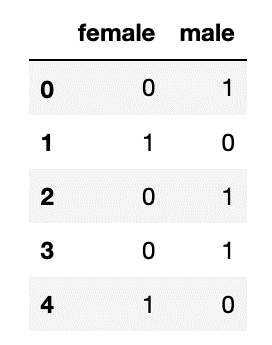
\includegraphics{./pic/chapter-2-1_pic_0.png}
\caption{chapter-2-1\_pic\_0.png}
\end{figure}

    Similar to the MinMaxScaler class, scikit-learn also implements a class
for standardization:

    \begin{tcolorbox}[breakable, size=fbox, boxrule=1pt, pad at break*=1mm,colback=cellbackground, colframe=cellborder]
\prompt{In}{incolor}{23}{\boxspacing}
\begin{Verbatim}[commandchars=\\\{\}]
\PY{k+kn}{from} \PY{n+nn}{sklearn}\PY{n+nn}{.}\PY{n+nn}{preprocessing} \PY{k+kn}{import} \PY{n}{StandardScaler}

\PY{n}{stdsc} \PY{o}{=} \PY{n}{StandardScaler}\PY{p}{(}\PY{p}{)}
\PY{n}{df4} \PY{o}{=} \PY{n}{pd}\PY{o}{.}\PY{n}{DataFrame}\PY{p}{(}\PY{n}{stdsc}\PY{o}{.}\PY{n}{fit\PYZus{}transform}\PY{p}{(}\PY{n}{df2}\PY{p}{)}\PY{p}{)}
\PY{n}{df4}
\end{Verbatim}
\end{tcolorbox}

            \begin{tcolorbox}[breakable, size=fbox, boxrule=.5pt, pad at break*=1mm, opacityfill=0]
\prompt{Out}{outcolor}{23}{\boxspacing}
\begin{Verbatim}[commandchars=\\\{\}]
          0         1         2         3         4         5
0 -1.170242 -1.359724 -1.189131 -1.041783 -0.920815 -0.824435
1 -1.601005 -1.210304 -1.102065 -0.994071 -0.895974 -0.812022
2 -1.601005 -0.986174 -0.958907 -0.908042 -0.846835 -0.785069
3  0.050256 -0.612623 -0.686823 -0.721391 -0.725003 -0.708630
4  1.198959 -0.239072 -0.372880 -0.473014 -0.538122 -0.573535
5  0.768195  0.134478 -0.017078 -0.154092 -0.266345 -0.351091
6  0.696401  0.508029  0.380582  0.244194  0.112820 -0.004480
7  0.624608  0.881579  0.820102  0.730661  0.624511  0.512260
8  0.337432  1.255130  1.301481  1.314127  1.296512  1.255243
9  0.696401  1.628681  1.824719  2.003411  2.159252  2.291760
\end{Verbatim}
\end{tcolorbox}
        
    \hypertarget{dimensionality-reduction}{%
\subsection{Dimensionality Reduction}\label{dimensionality-reduction}}

    \hypertarget{principal-component-analysis-pca}{%
\subsubsection{Principal Component Analysis
(PCA)}\label{principal-component-analysis-pca}}

    PCA as a concept is useful for measuring risk arising from a set of
correlated market variables. For example, interest rates that are quoted
in the market have correlation to each other. Thus, an interest rate for
tenor 1Y is not independent of interest rate for tenor say 3Y. There is
always some degree of correlation between all the tenor points with each
other. To achieve this objective, the PCA model computes a set of
variables that are called as Principal components (PCs). PCA is a model
which involves transforming a set of observations (i.e.~interest rate
time series in our case) into a set of uncorrelated variables called as
the PCs. This transformation behaves in way such that the first PC
explains the largest possible variance, and this accounts for majority
of the variability in the data. Each succeeding component in turn
explains the highest possible variance while at the same time following
the condition of orthogonality to each of the preceding PCs.

    \begin{figure}
\centering
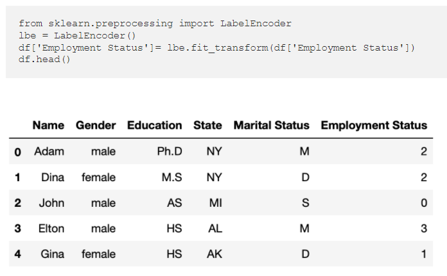
\includegraphics{./pic/chapter-2-1_pic_1.png}
\caption{chapter-2-1\_pic\_1.png}
\end{figure}

    Resulting PCs computed by the model are uncorrelated to each other,
thereby allowing them to be used independently with respect to each
other. Individual PCs are calculated using the concept of Eigen values
again a concept of linear algebra. PCs represent directions of the data
that explain the maximum amount of variance, i.e.~the vectors that
capture most of the information that is embedded in the data. The
relationship between the variance and information is that, the larger
the variance carried by the vector, the larger the dispersion of the
data points along it, and larger the dispersion along the vector, the
more information it contains.

PCA algorithm performs \textbf{dimensionality reduction} on the data
set. \textbf{\emph{Dimensionality reduction implies, we attempt to
capture the essence of a multivariate dataset into fewer number of
variables that would explain the required result}}.

So subsequent to generation of individual PCs, only those PCs are
selected that explain the maximum variation thereby capturing the
essence of the analysis. Machine learning algorithms implementing the
concept of Principal Component Analysis (PCA) can be used to this end. A
PCA algorithm accepts all of the incoming interest data as an input, and
it processes the data so that as an output we get a certain set of
interest rate tenor points which contribute to around say 97\% to 98\%
of the risk of our interest rate sensitive portfolio. This is
technically termed as dimensionality reduction as mentioned earlier.
This substantially reduces the load on the system resources, since now,
the system will use only those tenor points as have been chosen by the
PCA algorithm. This enables freeing up of valuable system resources
which now can be used for other productive purposes. PCA can be
implemented in Python.

PCA algorithm involves the following steps:

\begin{enumerate}
\def\labelenumi{\arabic{enumi}.}
\tightlist
\item
  \textbf{Standardization}: As we have already seen in this notebook,
  this step involves standardizing the input variables so that they may
  be used in the PCA analysis. Accuracy of PCA algorithm is a function
  of the accuracy of inputs. So, in the very first step of the
  algorithm, we perform a standardization which results in all variables
  getting transformed to a same scale. This builds the foundation of the
  PCA analysis.
\item
  \textbf{Covariance matrix}: This step involves computation of a
  covariance matrix which gives the relationship between the input
  variables. A covariance matrix is a symmetric matrix. With the
  diagonal elements giving the correlation, and the off-diagonal
  elements giving the covariance between variables. Depending on the
  sign of the covariance, the algorithm understands whether there is a
  direct or an inverse relation between variables. This step is
  important with respect to dimensionality reduction, as highly
  correlated variables may convey redundant information so the algorithm
  may appropriately handle these during the analysis.
\item
  \textbf{Eigen algebra}: Eigen values and Eigen vectors are calculated
  from the covariance matrix computed in the step above. Eigenvectors of
  the covariance matrix are the direction of the axes where there is
  most variance i.e.~most information. These are the PCs. Eigen values
  are the coefficients attached to the eigen vectors; they explain the
  amount of variance carried by each of the PCs. By ranking the eigen
  vectors in the order of their eigen values, we get the PCs in order of
  their significance. Next, we choose only the top 2 or top 3 PCs. The
  reason being, that its these top 2 or top 3 PCs that explain most of
  the variance in the data. Generally, top 3 PCs explain more than 97\%
  of the variance in the data. Speaking about \textbf{Interest Rate
  Risk}, out of the top 3 PCs the first PC is attributed to account for
  parallel shifts in the rates, second PC is attributed to account for
  steepening of the curve, third PC is attributed to account for bowing
  of the interest rate curve. We also compute the standard deviations of
  the same called as factor loadings.
\end{enumerate}

    \begin{tcolorbox}[breakable, size=fbox, boxrule=1pt, pad at break*=1mm,colback=cellbackground, colframe=cellborder]
\prompt{In}{incolor}{1}{\boxspacing}
\begin{Verbatim}[commandchars=\\\{\}]
\PY{k+kn}{import} \PY{n+nn}{numpy} \PY{k}{as} \PY{n+nn}{np}
\PY{k+kn}{import} \PY{n+nn}{pandas} \PY{k}{as} \PY{n+nn}{pd}
\PY{k+kn}{from} \PY{n+nn}{sklearn}\PY{n+nn}{.}\PY{n+nn}{decomposition} \PY{k+kn}{import} \PY{n}{PCA}
\PY{k+kn}{from} \PY{n+nn}{sklearn}\PY{n+nn}{.}\PY{n+nn}{preprocessing} \PY{k+kn}{import} \PY{n}{scale}
\end{Verbatim}
\end{tcolorbox}

    \begin{tcolorbox}[breakable, size=fbox, boxrule=1pt, pad at break*=1mm,colback=cellbackground, colframe=cellborder]
\prompt{In}{incolor}{23}{\boxspacing}
\begin{Verbatim}[commandchars=\\\{\}]
\PY{c+c1}{\PYZsh{}}
\PY{c+c1}{\PYZsh{} Here we have to load the file \PYZsq{}MarketData.csv\PYZsq{}}
\PY{c+c1}{\PYZsh{}}
\PY{k}{if} \PY{l+s+s1}{\PYZsq{}}\PY{l+s+s1}{google.colab}\PY{l+s+s1}{\PYZsq{}} \PY{o+ow}{in} \PY{n+nb}{str}\PY{p}{(}\PY{n}{get\PYZus{}ipython}\PY{p}{(}\PY{p}{)}\PY{p}{)}\PY{p}{:}
    \PY{k+kn}{from} \PY{n+nn}{google}\PY{n+nn}{.}\PY{n+nn}{colab} \PY{k+kn}{import} \PY{n}{files}
    \PY{n}{uploaded} \PY{o}{=} \PY{n}{files}\PY{o}{.}\PY{n}{upload}\PY{p}{(}\PY{p}{)}
    \PY{n}{path} \PY{o}{=} \PY{l+s+s1}{\PYZsq{}}\PY{l+s+s1}{\PYZsq{}}
\PY{k}{else}\PY{p}{:}
    \PY{n}{path} \PY{o}{=} \PY{l+s+s1}{\PYZsq{}}\PY{l+s+s1}{./data/}\PY{l+s+s1}{\PYZsq{}}
\end{Verbatim}
\end{tcolorbox}

    \begin{tcolorbox}[breakable, size=fbox, boxrule=1pt, pad at break*=1mm,colback=cellbackground, colframe=cellborder]
\prompt{In}{incolor}{24}{\boxspacing}
\begin{Verbatim}[commandchars=\\\{\}]
\PY{n}{data} \PY{o}{=} \PY{n}{pd}\PY{o}{.}\PY{n}{read\PYZus{}csv}\PY{p}{(}\PY{n}{path} \PY{o}{+} \PY{l+s+s1}{\PYZsq{}}\PY{l+s+s1}{MarketData.csv}\PY{l+s+s1}{\PYZsq{}}\PY{p}{,} \PY{n}{sep}\PY{o}{=}\PY{l+s+s1}{\PYZsq{}}\PY{l+s+s1}{,}\PY{l+s+s1}{\PYZsq{}}\PY{p}{)}
\PY{n}{x} \PY{o}{=} \PY{n}{pd}\PY{o}{.}\PY{n}{DataFrame}\PY{p}{(}\PY{n}{data}\PY{p}{)}
\PY{n}{x}\PY{o}{.}\PY{n}{head}\PY{p}{(}\PY{p}{)}
\end{Verbatim}
\end{tcolorbox}

            \begin{tcolorbox}[breakable, size=fbox, boxrule=.5pt, pad at break*=1mm, opacityfill=0]
\prompt{Out}{outcolor}{24}{\boxspacing}
\begin{Verbatim}[commandchars=\\\{\}]
   Date    3m    6m    1y    2y    3y    4y    5y    7y   10y
0     1  7.71  7.90  8.16  8.56  8.71  8.75  8.94  9.04  8.76
1     2  7.75  7.93  8.17  8.58  8.72  8.76  8.96  9.05  8.76
2     3  7.68  7.90  8.18  8.54  8.69  8.75  8.92  9.02  8.73
3     4  7.69  7.93  8.22  8.55  8.70  8.76  8.93  9.03  8.75
4     5  7.69  7.96  8.22  8.55  8.70  8.76  8.93  9.03  8.75
\end{Verbatim}
\end{tcolorbox}
        
    \begin{tcolorbox}[breakable, size=fbox, boxrule=1pt, pad at break*=1mm,colback=cellbackground, colframe=cellborder]
\prompt{In}{incolor}{25}{\boxspacing}
\begin{Verbatim}[commandchars=\\\{\}]
\PY{n}{df} \PY{o}{=} \PY{n}{x}\PY{o}{.}\PY{n}{drop}\PY{p}{(}\PY{n}{axis}\PY{o}{=}\PY{l+m+mi}{1}\PY{p}{,}\PY{n}{columns}\PY{o}{=}\PY{p}{[}\PY{l+s+s1}{\PYZsq{}}\PY{l+s+s1}{Date}\PY{l+s+s1}{\PYZsq{}}\PY{p}{]}\PY{p}{)}
\PY{n}{X} \PY{o}{=} \PY{n}{df}\PY{o}{.}\PY{n}{values}
\end{Verbatim}
\end{tcolorbox}

    \begin{tcolorbox}[breakable, size=fbox, boxrule=1pt, pad at break*=1mm,colback=cellbackground, colframe=cellborder]
\prompt{In}{incolor}{17}{\boxspacing}
\begin{Verbatim}[commandchars=\\\{\}]
\PY{c+c1}{\PYZsh{}Normalization of the data}
\PY{n}{X} \PY{o}{=} \PY{n}{scale}\PY{p}{(}\PY{n}{X}\PY{p}{)}
\end{Verbatim}
\end{tcolorbox}

    Factor loadings can be calculated as below:

    \begin{tcolorbox}[breakable, size=fbox, boxrule=1pt, pad at break*=1mm,colback=cellbackground, colframe=cellborder]
\prompt{In}{incolor}{19}{\boxspacing}
\begin{Verbatim}[commandchars=\\\{\}]
\PY{n}{pca} \PY{o}{=} \PY{n}{PCA}\PY{p}{(}\PY{n}{n\PYZus{}components}\PY{o}{=}\PY{l+m+mi}{9}\PY{p}{)}
\PY{n}{pca}\PY{o}{.}\PY{n}{fit}\PY{p}{(}\PY{n}{X}\PY{p}{)}
\PY{n}{factor\PYZus{}loading} \PY{o}{=} \PY{n}{pca}\PY{o}{.}\PY{n}{components\PYZus{}}
\PY{n}{df\PYZus{}factor\PYZus{}loading} \PY{o}{=} \PY{n}{pd}\PY{o}{.}\PY{n}{DataFrame}\PY{p}{(}\PY{n}{factor\PYZus{}loading}\PY{p}{)}
\PY{n}{df\PYZus{}factor\PYZus{}loading}
\end{Verbatim}
\end{tcolorbox}

            \begin{tcolorbox}[breakable, size=fbox, boxrule=.5pt, pad at break*=1mm, opacityfill=0]
\prompt{Out}{outcolor}{19}{\boxspacing}
\begin{Verbatim}[commandchars=\\\{\}]
          0         1         2         3         4         5         6  \textbackslash{}
0 -0.326333 -0.332127 -0.335253 -0.336409 -0.336407 -0.336645 -0.336749
1  0.544483  0.481083  0.254532  0.026220 -0.094576 -0.232499 -0.195293
2 -0.420097 -0.089586  0.239718  0.367905  0.368985  0.193024  0.162056
3 -0.483507  0.155548  0.552238  0.194323 -0.150791 -0.285729 -0.310074
4 -0.077813  0.031178 -0.068074 -0.189461 -0.066528  0.199704  0.509370
5  0.265687 -0.373126 -0.286407  0.548879  0.267776  0.002223 -0.390429
6  0.156875 -0.313745  0.089269  0.445102 -0.474288 -0.417560  0.506926
7 -0.113533  0.227273 -0.269583 -0.058133  0.562689 -0.692176  0.238268
8  0.269520 -0.579435  0.541370 -0.417573  0.318277 -0.142704  0.020379

          7         8
0 -0.331415 -0.328477
1 -0.439282 -0.335432
2 -0.254609 -0.598480
3 -0.106423  0.432952
4 -0.714587  0.371542
5 -0.316872  0.286948
6  0.089134 -0.081522
7  0.028055  0.078216
8 -0.035621  0.028572
\end{Verbatim}
\end{tcolorbox}
        
    Factor loadings explain the relation between the impact of a factor on
interest rates at respective tenor points. In PCA we also analyse the
amount of dispersion explained by each of the PCs. Now we will see which
PC contributes how much amount of variance/dispersion:

    \begin{tcolorbox}[breakable, size=fbox, boxrule=1pt, pad at break*=1mm,colback=cellbackground, colframe=cellborder]
\prompt{In}{incolor}{22}{\boxspacing}
\begin{Verbatim}[commandchars=\\\{\}]
\PY{c+c1}{\PYZsh{} variance percent of each PC}
\PY{n}{variance\PYZus{}percent\PYZus{}df} \PY{o}{=} \PY{n}{pd}\PY{o}{.}\PY{n}{DataFrame}\PY{p}{(}\PY{n}{data}\PY{o}{=}\PY{n}{pca}\PY{o}{.}\PY{n}{explained\PYZus{}variance\PYZus{}}\PY{p}{)}
\PY{n}{variance\PYZus{}ratio\PYZus{}df} \PY{o}{=} \PY{n}{pd}\PY{o}{.}\PY{n}{DataFrame}\PY{p}{(}\PY{n}{data}\PY{o}{=}\PY{n}{pca}\PY{o}{.}\PY{n}{explained\PYZus{}variance\PYZus{}ratio\PYZus{}}\PY{p}{)}
\PY{n}{variance\PYZus{}ratio\PYZus{}df} \PY{o}{=} \PY{n}{variance\PYZus{}ratio\PYZus{}df} \PY{o}{*} \PY{l+m+mi}{100}
\PY{n}{variance\PYZus{}ratio\PYZus{}df}
\end{Verbatim}
\end{tcolorbox}

            \begin{tcolorbox}[breakable, size=fbox, boxrule=.5pt, pad at break*=1mm, opacityfill=0]
\prompt{Out}{outcolor}{22}{\boxspacing}
\begin{Verbatim}[commandchars=\\\{\}]
           0
0  96.406078
1   1.931193
2   1.183464
3   0.242575
4   0.125015
5   0.059899
6   0.032387
7   0.013283
8   0.006106
\end{Verbatim}
\end{tcolorbox}
        
    From the table alongside, we observe that PC1 explains almost 96\% of
the total variation, and PC2 explains close to 1.95\% of total
variation. Therefore, rather than using all PCs in the subsequent
calculation, we can only use PC1 and PC2 in further calculation as these
two components explain close to 98\% of the total variance.

\begin{itemize}
\tightlist
\item
  PC1 corresponds to the roughly the parallel shift in the yield curve.
\item
  PC2 corresponds to roughly a steepening in the yield curve.
\end{itemize}

This is in-line with the theory of fixed income risk measurement which
states that majority of the movement in the price of a bond is explained
by the parallel shift in the yield curve and the residual movements in
the price is explained by steepening and curvature of the interest rate
curve.

    \hypertarget{references}{%
\subsection{References}\label{references}}

    \textbf{Abhyankar Ameya}, ``\emph{Exploring Risk Analytics using PCA
with Python}'',
\href{https://abhyankar-ameya.medium.com/exploring-risk-analytics-using-pca-with-python-3aca369cbfe4}{Medium},
data files for the interest rate example and further details about the
python code can be dowloaded from the github repository of the author
\href{https://github.com/Ameya1983/TheAlchemist}{here}


    % Add a bibliography block to the postdoc
    
    
    
\end{document}
